% id: 91-19
% book: 쎈B 공통수학2 · 07 명제
% section: 유형 06 명제의 참, 거짓과 진리집합
% figure: tikz:fig-91-19
% answer: 
% answer_source: 
% variant_level: 0 (원본 전사)
% 이 파일은 build.mjs 가 items.json 에서 만든다. 고칠 때는 items.json 을 고친다.
\smash{\raisebox{1.5mm}{\dmkichul{쎈B 공통수학2 91쪽 19번}}}
\noindent\begin{minipage}[t]{0.58\linewidth}\vspace{0pt}\raggedright 전체집합 $U$에 대하여 세 조건 $p$, $q$, $r$의 진리집합을 각각 $P$, $Q$, $R$라 할 때, 세 집합 $P$, $Q$, $R$ 사이의 포함 관계는 오른쪽 그림과 같다. 다음 중 거짓인 명제는?\end{minipage}\hfill\begin{minipage}[t]{0.4\linewidth}\vspace{0pt}\centering \resizebox{\ifdim\width>\linewidth\linewidth\else\width\fi}{!}{% 91-19(91쪽) — 전체집합 U 안의 세 진리집합 P, Q, R 벤 다이어그램. 원 P 안에 작은 원 Q 가 들어 있고 원 R 는 P 와 떨어져 있다.
% 스캔 화질이 낮아 TikZ 로 다시 그림. 라벨은 원문 그대로 U·P·Q·R 만 두고 보기 ①~⑤ 중 거짓인 명제(답)는 적지 않는다.
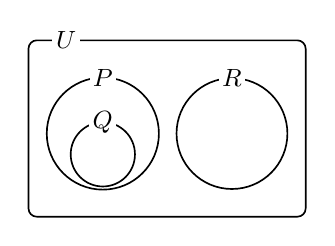
\begin{tikzpicture}[scale=0.8, line width=0.5pt, every node/.style={font=\small}]
  \draw[line width=0.6pt, rounded corners=3pt] (-2.2,-1.4) rectangle (2.2,1.4);
  \node[fill=white, inner sep=1.5pt] at (-1.6,1.4) {$U$};
  \draw[line width=0.6pt] (-1.02,-0.08) circle (0.89);
  \draw[line width=0.6pt] (-1.02,-0.41) circle (0.51);
  \draw[line width=0.6pt] (1.03,-0.08) circle (0.88);
  \node[fill=white, inner sep=1.2pt] at (-1.02,0.81) {$P$};
  \node[fill=white, inner sep=1.2pt] at (-1.02,0.10) {$Q$};
  \node[fill=white, inner sep=1.2pt] at (1.03,0.80) {$R$};
\end{tikzpicture}
}\end{minipage}\par
\begin{choices32}{$p\longrightarrow {\sim} r$}{$q\longrightarrow p$}{$r\longrightarrow {\sim} q$}{${\sim} p\longrightarrow {\sim} q$}{${\sim} q\longrightarrow {\sim} r$}\end{choices32}
